\documentclass[11pt,a4paper]{report}
\usepackage[utf8]{inputenc}
\usepackage[T1]{fontenc}
\usepackage{alltt}
\usepackage{graphicx}
\usepackage{hyperref}
\usepackage{scrextend}
\usepackage{enumitem}

% Changed the section command to say "Task #"
\def\thesection{Task \arabic{section}:}
% Added a familiar HTML command for new paragraph
\newcommand{\p}{\medskip\noindent}

% Meta, should be edited and filled in with relative information
\title{TDT4230 Graphics and Visualisation \\ Assignment 2}

\author{Nikola Dordevic}
\date{\today}

\begin{document}
\maketitle
% Use \section for tasks
\section{Fontastic decorations}
\begin{enumerate}[label=(\alph*)]\setcounter{enumi}{10}
	\item \hfill
	
	\begin{figure}[h]
		\centering
		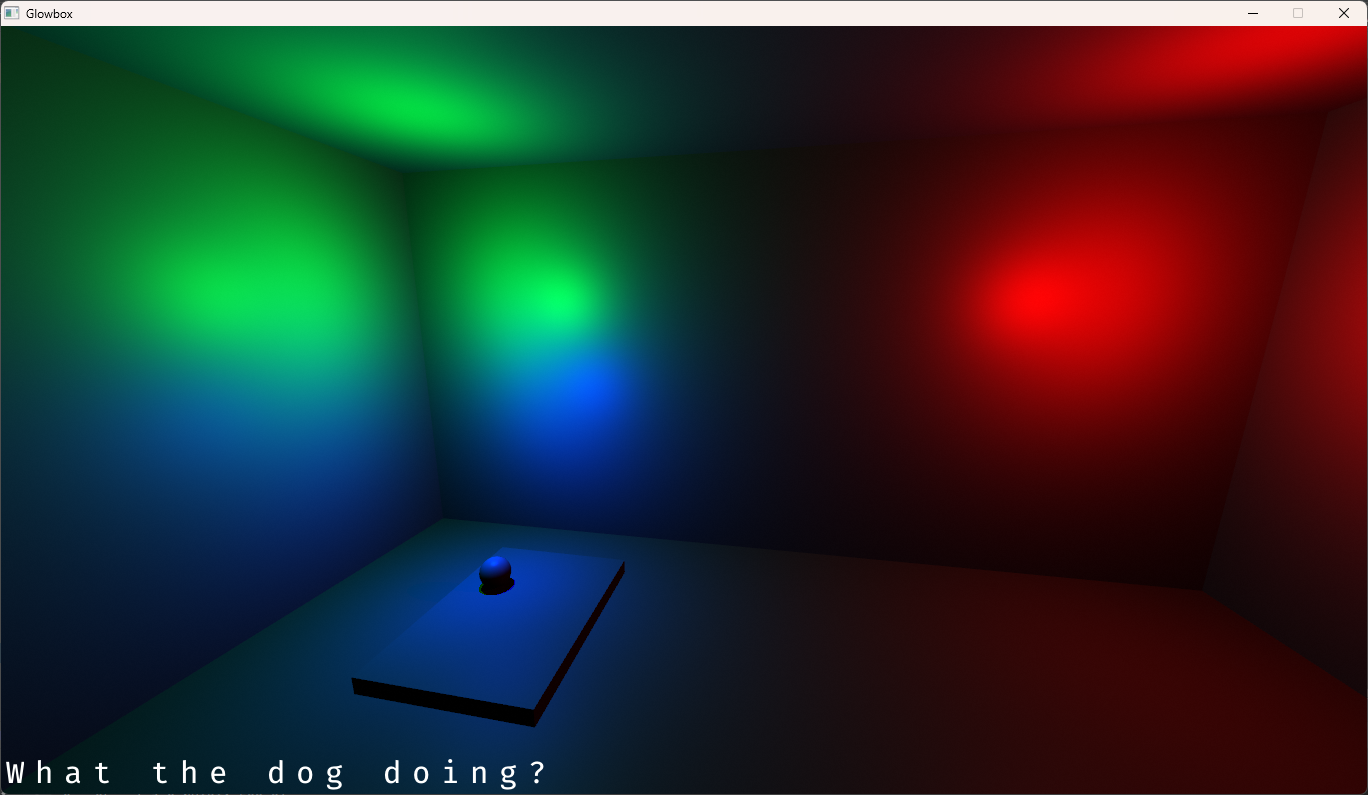
\includegraphics[width=\textwidth]{images/task1k.png}
		\caption{Screenshot of Glowbox with rendered text}
	\end{figure}
\end{enumerate}

% Command for next page
\clearpage

\section{Colourful Questions}
\begin{enumerate}[label=(\alph*)]\setcounter{enumi}{0}
	\item If we were to use linear interpolation the rendered texture will look distorted when vertices have different depths, and it will be increasingly obvious the closer the texture is to the diagonal.
	
	This is because the ratios between different points in the texture are not preserved in perspective projection.
	If we were to imagine a texture where one side is further back in the room while the other is closer, through the perspective projection, points further back the texture would look closer together than those in the front, even though all points in the texture are equispaced, which is why the interpolation has to be non-linear.
	
	\item \begin{enumerate}[label=(\alph*)]\setcounter{enumi}{0}
		\item A displacement map displaces the geometry on the surface of a given object. This would not work on our walls because there are far to few polygons in the wall to displace.
		\item To reap the benefits of a displacement map we would have to perform tesselation or subdivision on the surface. This will effectively increase the level of detail on the surface, enabling us to use the displacement map as intended. \end{enumerate}

	\item[(c)] Mip-mapping recursively filters and down-samples textures into smaller versions of themselves. From the Texture slides, it is mentioned that a 2x2 box filter is used for overaging the parent texels to produce the next version of the map.
	In the given scenario this would cause the green side of the texture to bleed into the hypotenuse of the two red triangles, causing the diagonal of the rectangle to have some green in it.
	
	
	
\end{enumerate}

\clearpage


\section{Abnormal normals}

\end{document}